% \documentclass[addpoints,12pt]{exam}
\documentclass[addpoints,answers,12pt]{exam}

\usepackage{ifthen}

\ifthenelse{\equal{\includedsol}{solution}} 
{ 
\printanswers
} 
{ 
\noprintanswers
} 

%%%%%%%%%%%%%%%%%%%%%%%%%%%%%%%%%%%%%%%%%%%%%%%%%%%%%%%%%%%%%%%%
%% To flush left insert:
% \begin{flushleft}
% \end{flushleft}


\usepackage{graphics}
\usepackage{epsf}
\usepackage{epsfig}
\usepackage{enumerate}

% \usepackage{amsgen}
% \usepackage{amstext}
% \usepackage{amsmath}
% % \usepackage{amsthm}
% \usepackage{amsfonts}


\usepackage{latexsym}
\usepackage{amsgen}
\usepackage{amsmath}
\usepackage{amstext}
\usepackage{amscd}
\usepackage{amssymb}


% \setlength\answerclearance{0.6ex}
\firstpageheader{CSE 344
}{Midterm}{Name:\enspace\makebox[2in]{\hrulefill}} \runningheader{CSE
  344}{Midterm}{Nov. 7, 2012}



\newcommand{\eat}[1]{}

\begin{document}

\title{CSE 344  Midterm}
\author{}
\date{Wednesday, November 7, 2012, 9:30-10:20}

\maketitle

\begin{center}
{
\vspace{1cm}

{\LARGE Name:\enspace\makebox[3in]{\hrulefill}}


\vspace{1cm}

\gradetable
}
\end{center}

\begin{itemize}
\item This exam is open book and open notes but NO laptops or other portable devices.
\item You have 50 minutes; budget time carefully.
\item Please read all questions carefully before answering them.
\item Some questions are easier, others harder.  Plan to answer all
  questions, do not get stuck on one question. If you have no idea how to answer
a question, write your thoughts about the question for partial credit.
\item Good luck!
\end{itemize}

\newpage

\begin{questions}
\section{SQL and Physical Tuning}

\question (\totalpoints\ \points) 

You have been analyzing the data from a social
networking site and have derived the following relation,
which captures topics discussed by various users.

\begin{tabular}{l}
  \texttt{Discussion(\underline{user1,user2,topic})} \\
\end{tabular}

\eat{
drop table Discussion
create table Discussion(user1 varchar(50), user2 varchar(50), topic varchar(50))

insert into Discussion values ('Alice','Bob','TopicAlicBob1')
insert into Discussion values ('Alice','Bob','TopicAlicBob2')
insert into Discussion values ('Alice','Bob','TopicAlicBob3')
insert into Discussion values ('Alice','Chuck','TopicAlicChuck1')
insert into Discussion values ('Alice','Chuck','TopicAlicChuck2')
insert into Discussion values ('Bob','Chuck','TopicBobChuck1')
insert into Discussion values ('Alice','Chuck','TopicAlicBob1')
}

The relation contains a tuple \texttt{(u1,u2,t)} every time a user
\texttt{u1} discussed a topic \texttt{t} with user \texttt{u2}. To
avoid duplicate entries, \texttt{user1} always precedes \texttt{user2}
in alphabetical order.

\begin{parts}

  \part[15] Write a SQL query that returns all topics discussed by
  \texttt{Alice} and \texttt{Bob} but not discussed by \texttt{Alice}
  and \texttt{Chuck}.\vfill

\begin{solution}
\begin{verbatim}
select topic
from Discussion
where user1='Alice'
and user2='Bob'
and topic not in
    (select topic
     from Discussion
     where user1='Alice'
     and user2='Chuck')
\end{verbatim}
\end{solution}


\newpage

{\scriptsize
\hfill
\begin{tabular}{l}
  \texttt{Discussion(\underline{user1,user2,topic})} \\
\end{tabular}
}

\part[15] Write a SQL query that returns the number
of topics discussed by more than 10 pairs of users.  \vfill

\begin{solution}
\begin{verbatim}
select count(*)
from 
  ( select topic 
    from Discussion
    group by topic
    having( count(*) > 10 ) as X
  )
\end{verbatim}

\end{solution}

\newpage


\part[5] Give two reasons why database administrators typically 
do \textbf{NOT} create an index on every single attribute of every
single relation. You do not need to discuss the reasons. Just
state them.

\vfill

\begin{solution}
\begin{enumerate}
\item Reason 1: Indexes take-up space
\item Reason 2: Indexes can slow-down updates (inserts, deletes, updates)
\end{enumerate} 
\end{solution}

\newpage

\part[10] Explain how a database administrator should proceed in order
to select a good set of indexes for a relational database. Note that
more complete answers will receive more points.

\vfill

\begin{solution}
  The DBA should first talk to the developers and users to determine
  the \textbf{workload}, in the form of a set of \textbf{queries,
    updates, and their frequencies}, that needs to execute on the
  database. The DBA should then consider which indexes have the
  potential to speed-up the queries in the workload. He or she should
  consider the most frequent (or otherwise most important) queries
  first. When selecting the indexes, the DBA should consider the
  \textbf{trade-off between slowing down updates, using space, and
    accelerating queries}. The DBA should also consider which indexes
  should be \textbf{clustered and which ones should be unclustered}.
  For each relation, only one index can be clustered.
\end{solution}


\end{parts}
\newpage

\section{Relational Algebra, Datalog, and Relational Calculus}

\question (\totalpoints\ \points) 

Consider the following database schema. Relation \texttt{Clinic} lists
medical clinics with their unique identifiers, names, street
addresses, and states. Relation \texttt{Equipment} lists the unique
identifiers, types, and models of various pieces of
equipment. Finally, relation \texttt{Assignment} indicates the
equipment available in each clinic.

\begin{tabular}{l}
  \texttt{Clinic(\underline{cid}, name, street, state)} \\
  \texttt{Equipment(\underline{eid}, type, model)} \\
  \texttt{Assignment(\underline{cid, eid})} \\
\end{tabular}

\newpage
\begin{parts}

  \part[10] Write a Relational Algebra expression in the form of a logical query
  plan that is equivalent to the SQL query below:

\begin{verbatim}
select count(*)
from Clinic C
where not exists
   (select * 
    from Assignment A, Equipment E
    where C.cid = A.cid 
    and   A.eid  = E.eid
    and   E.type = 'Fridge'
    and   E.model = 1004
   )
\end{verbatim}

\vfill

\eat{
create table Clinic (cid int, name varchar(50), street varchar(50), state char(2))
create table Equipment (eid int, type varchar(50), model varchar(50))
create table Assignment (cid int, eid int)

insert into Equipment values (1, 'Fridge', '1004')
insert into Equipment values (2, 'Fridge', '1005')
insert into Equipment values (3, 'Fridge', '1006')
insert into Equipment values (4, 'Other', '1007')

insert into Clinic values (1, 'One', 'StreetOne', 'WA')
insert into Clinic values (2, 'Two', 'StreetTwo', 'WA')
insert into Clinic values (3, 'Three', 'StreetThree', 'MA')
insert into Clinic values (4, 'Four', 'StreetFour', 'MA')
insert into Clinic values (5, 'Five', 'StreetFive', 'NY')

insert into Assignment values (1, 1)
insert into Assignment values (2, 2)
insert into Assignment values (3, 3)
insert into Assignment values (4, 4)
insert into Assignment values (5, 1)

}

  \begin{solution}
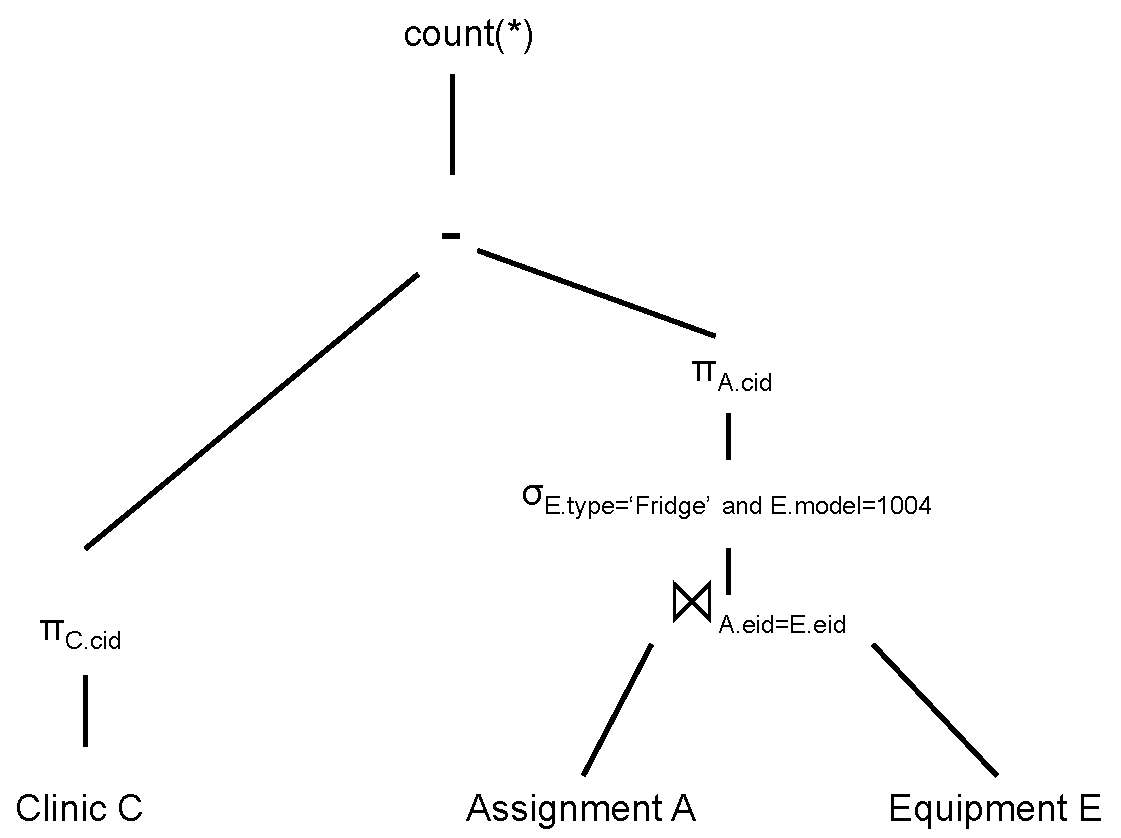
\includegraphics[width=0.5\linewidth]{relational-algebra.pdf}
  \end{solution}

\newpage

{\scriptsize
\hfill
\begin{tabular}{l}
  \texttt{Clinic(\underline{cid}, name, street, state)} \\
  \texttt{Equipment(\underline{eid}, type, model)} \\
  \texttt{Assignment(\underline{cid, eid})} \\
\end{tabular}
}

\part[10]  Write a Datalog query equivalent to the following SQL query:

\begin{verbatim}
select C.name
from Clinic C
where not exists
   (select * 
    from Assignment A, Equipment E
    where C.cid = A.cid 
    and   A.eid  = E.eid
    and  E.type = 'Fridge'
    and  E.model = 1004
   )
\end{verbatim}

\vfill

  \begin{solution}
AllClinics(x,y) :- Clinic(x,y,\_,\_)

NonAnswers(x)  :- Assignment(x,z),Equipment(z,'Fridge',1004)

Answer(y) :- AllClinics(x,y) NOT NonAnswers(x)
  \end{solution}

%\newpage

% {\scriptsize
% \hfill
% \begin{tabular}{l}
%   \texttt{Clinic(\underline{cid}, name, street, state)} \\
%   \texttt{Equipment(\underline{eid}, type, model)} \\
%   \texttt{Assignment(\underline{cid, eid})} \\
% \end{tabular}
% }

%   \part[5] Write a Datalog query that computes the names
% of all clinics that are either located in the state of WA or
% have been assigned at least two pieces of equipment of the
% same type.

% \vfill
% \begin{solution}
% \begin{verbatim}
% Answer(y) :- Clinic(\_,y,\_,'WA')
% Answer(y) :- Clinic(x,y,\_,\_), Equipment(v,t,\_), Assignment(x,v), Assignment(x,w), Equipment(w,t,\_)
% \end{verbatim}
% \end{solution}

\newpage

{\scriptsize
\hfill
\begin{tabular}{l}
  \texttt{Clinic(\underline{cid}, name, street, state)} \\
  \texttt{Equipment(\underline{eid}, type, model)} \\
  \texttt{Assignment(\underline{cid, eid})} \\
\end{tabular}
}

\part[10] Write a relational calculus query that returns the types
of equipment assigned to clinics in the state of \texttt{WA}:

\vfill

\begin{solution}
  \begin{align*}
Q(t) = \exists c. \exists n. \exists s. \exists e . \exists m. \left(\texttt{Clinic}(c,n,s,"WA") \wedge \texttt{Assignment}(c,e) \wedge \texttt{Equipment}(e,t,m) \right)
  \end{align*}
\end{solution}

\newpage

% \part[10] Write a relational calculus query that returns the
% types of equipment assigned to all clinics in WA

% \vfill

% \begin{solution}
%   \begin{align*}
% %    Q(u,n) = \texttt{Users}(u,n) \wedge \forall p.\forall  i.\left(\texttt{Picture}(p,u,i) \Rightarrow \forall v.\forall s.\forall  t.\left(\texttt{Comment}(v,p,s,t) \Rightarrow s > 5\right)\right)
%   \end{align*}
% \end{solution}

\end{parts}
\newpage

\section{XML and XPath}


\question (\totalpoints\ \points) 


\begin{parts}
  \part[15] Consider the following XML document stored in a file
called trips.xml:

\begin{verbatim}
<trips>
  <business reason='Meeting at CompanyX' destination='Baltimore'>
    <airline>American</airline>
    <stops>
      <location>Houston</location>
      <location>Boston</location>
    </stops>    
  </business>

  <personal destination='Boston'>
    <airline>American</airline>
    <stops>
      <location>Chicago</location>
    </stops>
  </personal>

  <personal destination='Hawaii'>
    <airline>Alaska</airline>
    <stops>
    </stops>
  </personal>

</trips>
\end{verbatim}

\newpage
Write an XQuery expression that will
transform it into the following document:

\begin{verbatim}
<trips>
  <airline>
    <name>American</name>
    <trip destination="Baltimore">
      <stops>2</stops>
    </trip>
    <trip destination="Boston">
      <stops>1</stops>
    </trip>
  </airline>
  <airline>
    <name>Alaska</name>
    <trip destination="Hawaii">
      <stops>0</stops>
    </trip>
  </airline>
</trips>
\end{verbatim}



\vfill
\begin{solution}
\begin{verbatim}
<trips>
{
  for $d in doc("trips.xml")/trips
  for $x in distinct-values( $d//airline/text())

  return 
    <airline>
      <name> {$x} </name>
      {
      for $y in $d/personal | $d/business 
      where $y/airline/text() = $x
      return 
           <trip> { $y/@destination } 
             <stops>{ count($y/stops/location) }</stops>
           </trip>
      }
   </airline>
}
</trips>
\end{verbatim}
\end{solution}

\newpage

\part[10] Write a possible DTD for the
document used as \textbf{input} above:

\vfill
\begin{solution}
\begin{verbatim}
<!DOCTYPE trips [
    <!ELEMENT trips  (business|personal)*>
    <!ELEMENT business (airline, stops)>
    <!ATTLIST business reason CDATA #REQUIRED >
    <!ATTLIST business destination CDATA #REQUIRED >
    <!ELEMENT personal (airline, stops)>
    <!ATTLIST personal destination CDATA #REQUIRED >
    <!ELEMENT airline  (#PCDATA )>
    <!ELEMENT stops    (location*)>
    <!ELEMENT location (#PCDATA )>
]>
\end{verbatim}
\end{solution}


\end{parts}

\end{questions}
\end{document}
